\documentclass[10pt]{article}
\usepackage[utf8]{inputenc}
\usepackage[papersize={11in, 17in}]{geometry}
\usepackage[absolute]{textpos}
\usepackage{graphicx}
\TPGrid[0.5in, 0.25in]{23}{24}
\usepackage{palatino}
\parindent=0pt
\parskip=12pt
\usepackage{nopageno}
\begin{document}

\begin{textblock}{23} (0, 1)
\center\huge PREFACE
\end{textblock}

\begin{textblock}{8} (0, 3)

\section{}

\textit{In vain, great-hearted Kublai, shall I attempt to describe Zaira, city
of high bastions. I could tell you how many steps make up the streets rising
like stairways, and the degree of the arcades' curves, and what kind of zinc
scales cover the roofs; but I already know this would be the same as telling
you nothing.} The city does not consist of this, but of relationships between
the measurements of its space and the events of its past: \textit{the height of
a lamppost and the distance from the ground of a hanged usurper's swaying feet;
the line strung from the lamppost to the railing opposite and the festoons that
decorate the course of the queen's nuptial procession; the height of that
railing and the leap of the adulterer who climbed over it at dawn; the tilt of
a guttering and a cat's progress along it as he slips into the same window; the
firing range of a gunboat which has suddenly appeared beyond the cape and the
bomb that destroys the guttering; the rips in the fish net and the three old
men seated on the dock mending nets and telling each other for the hundredth
time the story of the gunboat of the usurper, who some say was the queen's
illegitimate son, abandoned in his swaddling clothes there on the dock.}

\textit{As this wave from memories flows in, the city soaks it up like a sponge
and expands. A description of Zaira as it is today should contain all of
Zaira's past. The city, however, does not tell its past, but contains it like
the lines of a hand, written in the corners of the streets, the gratings of the
windows, the banisters of the steps, the antennae of the lightning rods, the
poles of the flags, every segment marked in turn with scratches, indentations,
scrolls. }

- Italo Calvino, \emph{Invisible Cities}

\end{textblock}

\begin{textblock}{14} (9, 3)

\section{Instrumentation}

\begin{itemize}

    \item[-] \textbf{Flute}, with shaker \\

    \item[-] \textbf{Oboe} \\

    \item[-] \textbf{Clarinet in b-flat}, with shaker \\

    \item[-] \textbf{Percussion} \\

        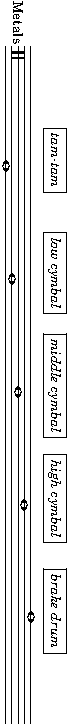
\includegraphics{preface-percussion-metals.pdf} \\ \\ \\
        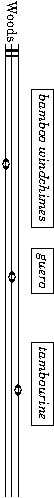
\includegraphics{preface-percussion-woods.pdf} \\ \\ \\
        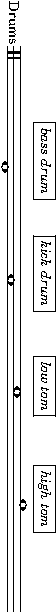
\includegraphics{preface-percussion-drums.pdf} \\

        Mallets: hard sticks or bare hands, wire brushes, superballs \\

    \item[-] \textbf{Piano} \\

        Prepare the strings in the lowest and highest octaves with any
        combination of felt, tape or rubber to dampen and distort the timbre of
        the strings. Putty-like substances work particularly well. \\

        Guero passages should be played with a piece of hard paper or
        plastic (e.g. a credit card), on the keys. 
        The register of the motions is left to the performer. \\

    \item[-] \textbf{Violin}, with shaker \\

    \item[-] \textbf{Viola}, with shaker \\

    \item[-] \textbf{Cello}

\end{itemize}

    Auxiliary shakers should be maracas, cabasas, brazil nut shakers or
    simliar. Uniform and disparate selections are equally interesting.

\end{textblock}


\end{document}
